
% !TeX root=DeepRelAttr.tex
% !TEX TS-program = pdfLatex

%%%%%%%%%%%%%%%%%%%%%%% END-TO-END DEEP RELATIVE ATTRIBUTES %%%%%%%%%%%%%%%
\section{Proposed Method}

%%%%%%%%%%%%%%%%%%%%%%%% Figure 2 %%%%%%%%%%%%%%%%%%%%%%%%%%%%%%%%%%%%%%%%%%%%%%%%%%%%%
\begin{figure*}
\label{fig.2}
\centering
\scalebox{.35}
{
% We need layers to draw the block diagram
\pgfdeclarelayer{background}
\pgfdeclarelayer{foreground}
\pgfsetlayers{background,main,foreground}

% Define a few styles and constants
\tikzstyle{sensor}=[draw, fill=blue!20, text width=5em, 
    text centered, minimum height=2.5em]
\tikzstyle{ann} = [above, text width=5em]
\tikzstyle{naveqs} = [sensor, text width=6em, fill=red!20, 
    minimum height=12em, rounded corners]
\def\blockdist{2.3}
\def\edgedist{2.5}

\begin{tikzpicture}
	% feature extraction part rectange
	\node [scale=3] (testtitle) at (10.5cm, 4.5cm) {Test time};
	\draw [rounded corners=1cm, dashed, line width=3, red] (-3.5cm, 4cm) rectangle (24.5cm,-2.5cm);
	% images
	\node (im1) at (0cm,1cm) [draw] {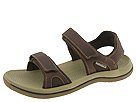
\includegraphics[scale=1]{im1.jpg}};
	\node (im2) at (0cm, -6cm) [draw] {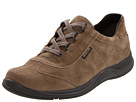
\includegraphics[scale=1]{im2.jpg}};

	% topconv1 layer
	\node (tconv1) at (5.1cm, 1cm) {};
%	\draw [fill=blue!20] (5.6cm,3.1cm) rectangle (9.6cm,0.1cm);
	\draw [fill=blue!20] (5.4cm,2.9cm) rectangle (9.4cm,-0.1cm);
	\draw [fill=blue!20] (5.2cm,2.7cm) rectangle (9.2cm,-0.3cm);
	\draw [fill=blue!20] (5cm,2.5cm) rectangle (9cm,-0.5cm);

	% bottomconv1 layer
	\node (bconv1) at (5.1cm, -6cm) {};
%	\draw [fill=blue!20] (5.6cm,-3.9cm) rectangle (9.6cm,-6.9cm);
	\draw [fill=blue!20] (5.4cm,-4.1cm) rectangle (9.4cm,-7.1cm);
	\draw [fill=blue!20] (5.2cm,-4.3cm) rectangle (9.2cm,-7.3cm);
	\draw [fill=blue!20] (5cm,-4.5cm) rectangle (9cm,-7.5cm);

	% arrows from images to conv1s
	\path [draw, ->, line width=3] (im1.east) -- node [above, scale=3] {$I_i$} (tconv1);
	\path [draw, ->, line width=3] (im2.east) -- node [above, scale=3] {$I_j$} (bconv1);

	% topconv2 layer
	\node (tconv2) at (12cm, 1cm) {};
	\draw [fill=blue!20] (12.6cm,3.1cm) rectangle (16.6cm,0.1cm);
	\draw [fill=blue!20] (12.4cm,2.9cm) rectangle (16.4cm,-0.1cm);
	\draw [fill=blue!20] (12.2cm,2.7cm) rectangle (16.2cm,-0.3cm);
	\draw [fill=blue!20] (12cm,2.5cm) rectangle (16cm,-0.5cm);

	% bottomconv2 layer
	\node (bconv2) at (12cm, -6cm) {};
	\draw [fill=blue!20] (12.6cm,-3.9cm) rectangle (16.6cm,-6.9cm);
	\draw [fill=blue!20] (12.4cm,-4.1cm) rectangle (16.4cm,-7.1cm);
	\draw [fill=blue!20] (12.2cm,-4.3cm) rectangle (16.2cm,-7.3cm);
	\draw [fill=blue!20] (12cm,-4.5cm) rectangle (16cm,-7.5cm);

	\path (tconv1.east)+(4.65cm, 0cm) -- node [scale=4]{\dots} (tconv2);
	\path (bconv1.east)+(4.65cm, 0cm) --node [scale=4]{\dots} (bconv2);

	\node (convnet) [below, scale=3.5] at (11cm, -8cm) {ConvNet};

	% toprank
	\node (tconvout) at (16.6cm, 1cm) {};
	\node (trank) at (20.5cm, 1cm) [rectangle, draw, fill=red!20, scale=3, align=center] {Ranking \\  Layer};
	\path [draw, line width=3, ->] (tconvout) -- node[above, scale=3] {$\psi_i$} (trank.west);

	% bottomrank
	\node (bconvout) at (16.6cm, -6cm) {};
	\node (brank) at (20.5cm, -6cm) [rectangle, draw, fill=red!20, scale=3, align=center] {Ranking \\  Layer};
	\path [draw, line width=3, ->] (bconvout) -- node[above, scale=3] {$\psi_j$} (brank.west);

	% shared rank layer
	\node (dashcenter) at (10.75cm, 0cm) {};
	\path [draw, line width=2, <->] (trank.south) -- node [scale=2, draw, rectangle, fill=white, line width=0] {\rotatebox{90}{shared}} (brank.north);
	\path [draw, line width=2, <->] (trank.south -| dashcenter) -- node [scale=2, draw, rectangle, fill=white, line width=0] {\rotatebox{90}{shared}} (brank.north -| dashcenter);

	% posterior
	\node (posterior) at (26cm, -2.5cm) [rectangle, draw, fill=orange!10, scale=3, minimum width=15] {\rotatebox{90}{Posterior}};

	% connect rank layer to posterior
	\path [draw, line width=2, ->] (trank.east) -- node [scale=3, above] {$r_i$} (posterior);
	\path [draw, line width=2, ->] (brank.east) -- node [scale=3, above] {$r_j$} (posterior);

	% BXE
	\node (bxent) at (33cm, -8cm) [draw,fill=green!10, regular polygon, regular polygon sides=3, shape border rotate=-90, scale=8, line width=2] {};
	\node at (33.2cm, -8cm) {\Huge BXEnt};

	% target value
	\node (target) at (26cm , -9.5cm) [scale=3] {target};

	% connect to bxe
	\draw [line width=3, ->] (posterior.east) -- ++(2cm, 0cm) |- node [above right, scale=3] {$p$}  (bxent.north west);
	\draw [line width=3, ->] (target.east) -- node [below, scale=3] {$t$}  (bxent.south west |- target.east);

	% loss node
	\node (loss) [scale=3] at (40cm, -8cm) { loss};

	% connect bxent to loss
	\draw [line width=3, ->] (bxent.east) --  (loss.west);
\end{tikzpicture}}
\end{figure*}
%%%%%%%%%%%%%%%%%%%%%%%% Figure 2 %%%%%%%%%%%%%%%%%%%%%%%%%%%%%%%%%%%%%%%%%%%%%%%%%%%%%

We propose to use a ConvNet based deep neural network that is trained to optimize the appropriate ranking loss for the task of predicting relative attribute strength. The network architecture consists of two parts, the \textit{feature extraction part} and the \textit{ranking part}.

The feature extraction part takes as input an image $I_i$ and outputs the feature representation of that image $\psi_i \in \mathbb{R}^d$ (Figure \cite{fig.2}).
As feature extraction part, some intermediate layer of any ConvNet architecture such as AlexNet \cite{krizhevski}, VGGNet \cite{verydeep} or GoogleNet \cite{googlenet}, can be used.

% In our experiments we use the fc7 (the last layer before the probability layer) of VGG-16 \cite{verydeep} as the feature extraction part of the network.

The ranking part, maps the feature representation $\psi_i$ to the attribute strength or absolute rank of the input $r_i \in \mathbb{R}$. Then given two attribute strengths generates the posterior $P_{ij}$ that the strength of the attribute in $I_i$ is larger than the strength of the attribute in $I_j$. 

\subsection{Learning to Rank Using Gradient Descent}


\subsection{Deep Relative Attributes}

